%
% The first command in your LaTeX source must be the \documentclass command.
\documentclass{article}

\usepackage[]{todonotes} % notes not showed
%% \usepackage[draft]{todonotes}   % notes showed

\usepackage{hyperref}
\usepackage{graphics}
\usepackage{multicol}

\newcommand{\blockchain}{{\ae}ternity blockchain}
\newcommand{\aet}{{\ae}ternity}

%
% \BibTeX command to typeset BibTeX logo in the docs
\AtBeginDocument{%
  \providecommand\BibTeX{{%
    \normalfont B\kern-0.5em{\scshape i\kern-0.25em b}\kern-0.8em\TeX}}}

\begin{document}

\title{DRAFT: The \blockchain\ \\white paper}

\author{Aeternity\\development team  \and Thomas Arts \and
             Yanislav Malahov \and Sascha Hanse}

\maketitle

%
% The abstract is a short summary of the work to be presented in the article.
\begin{abstract}
The \blockchain\ aims to be a development platform for advanced blockchain
applications that can be used by millions of users.
On the one hand the \blockchain\ is scalable due to a next generation
consensus algorithm and the use of state channels. On the other hand,
the \blockchain\ is a excellent development platform for
applications by offering native support for commonly used
blockchain features, as well as secure and highly efficient
contract language and virtual machine.

In this white paper we explain the above mentioned concepts of the
\blockchain\ and highlight the design decisions. The
paper provides a high-level overview of the technology. For detailed
and specific implementation details we refer to the \aet\ protocol
description.

\end{abstract}

%%\keywords{blockchain, state channels}

\newpage

\tableofcontents

\newpage

\section{Introduction}

Blockchain technology has been attracting significant attention since Bitcoin
was proposed by Nakamoto~\cite{SN} in 2008.
Many blockchain platforms are being developed to serve the next generation of
applications. The novelty of the field provides an interplay between developers
offering new features, enabling new applications to be written by application
developers, and application developers therewith requiring additional features
or possibilities.

Aeternity~\cite{AE,UlfWigerCodeMesh2018} is an open source blockchain
platform aiming to be a development platform for advanced blockchain
applications that can be used by millions of users. Several key technologies
are put in place to meet these scaling requirements, most notably state
channels, the next generation of Nakamoto consensus algorithm and the very
efficient FATE virtual machine for smart contract execution.

The platform runs as a decentralized trustless distributed ledger using
Proof-of-Work (PoW)~\cite{dwork1992pricing,back1997hashcash,Tromp2015CuckooCA}
for leader election.
In Sect.~\ref{sect:mining} we explain how we improve the scalability of
original Nakamoto consensus~\cite{SN} by leveraging
Bitcoin-NG~\cite{Eyal:2016:BSB:2930611.2930615}. The result of this change
is a throughput of about 100 on-chain transactions per second with
low latency as opposed to the seven transactions per second of Bitcoin.

Further increases in transaction throughput, possibly thousands of
transactions per second, can be achieved via state channels (Sect.\
\ref{sect:channels}),
an off-chain encrypted peer-to-peer communication protocol. After
agreeing on-chain to collaborate in a state channel, parties communicate
mutually authenticated transactions to each other. These transactions don't
have to be recorded on chain and thus can be exchanged at much higher
speed. Closing the channel, with or without dispute resolution, is performed
on-chain again.

The \blockchain\ offers a variety of different transaction types
based on commonly used applications on other blockchain implementations.
For example, by identifying that many blockchains have a need to give human
readable, persistent names to objects on chain, the \blockchain\ provides a
set of transactions that make this easy for developers, without the need to
implement a smart contract for it (\ref{sect:aens}). Another example is a set
of transactions to register and query oracles, which provide data from outside
the blockchain.
These transactions are explained in more detail in Sect.~\ref{sect:transactions}.

Many features are yet to be invented, but can already be implemented
by users if they use the \aet\ smart contract language
\textit{Sophia}. Sophia is a Turing complete functional language
designed with security in mind. Many mistakes that one can make in
other contract languages are impossible to make or are easier to detect
when using Sophia. In Sect.\ \ref{sect:sophia} we present some key
ideas of the language.

Contracts are compiled to bytecode, which is executed on a highly
efficient virtual machine \textit{FATE}. Similar to other smart contract
languages every operation has a gas cost associated to it. This cost reflects
the amount of work needed to execute a contract. The FATE virtual machine is
specifically designed for
\aet\ to meet the high security and efficiency demands, which we
explain in more detail in Sect.~\ref{sect:fate}.

The reference implementation of the \aet\ protocol is written using the
functional language Erlang~\cite{Armstrong:2010:ERL:1810891.1810910}. This
language originates from the telecommunication industry and is used in large
distributed and concurrent systems (e.g.\ WhatsApp). However, the choice
of implementation language has no further implications for the techniques used
and described in this paper.

\section{Mining Next Generation}
\label{sect:mining}

Traditionally blocks in a blockchain contain an ordered list of transactions
combined with a cryptographic hash ---Blake2b \cite{aumasson2013blake2} in our
case--- of the previous block \cite{whatisablockchain,raikwar2019sok} and mining
is the act of creating such blocks. Transactions are only added with the
creation of a new block which. In \cite{Eyal:2016:BSB:2930611.2930615}
Ittay et al. propose to decouple the leader election from inclusion of
transactions in blocks for scalability purposes. Their scheme dubbed
\enquote{Bitcoin-NG} is what we adopted using Cuckoo Cycle for proof-of-work.

% Chaining of hashes prevents that blocks can be tampered with. If a block
%changes with even one bit, the hash of the block will change.
%The changed block's successor will then contain the hash of a non-existing
%block. Thus, an attacker modifying a transaction in a block will also have to
%modify all consecutive blocks. Since the hashes also have to satisfy a
%difficulty requirement, which requires a non-trivial amount of work, rewriting
%a block in the history of the chain is assumed to require more computational
%resources than available to an attacker.

\subsubsection{Cuckoo Cycle PoW}

\textit{Cuckoo Cycle} \cite{Tromp2015CuckooCA}, a graph-theoretic problem of
finding cycles in a graph, is used for proof-of-work puzzles. Finding solutions
to this problem is memory bound, meaning that runtime is constrained by memory
latency of accessing nodes of the graph. Cuckoo cycle was chosen because memory
latency is believed to not allow as big performance gains from specialised
integrated circuits (ASICs) versus general purpose hardware. Verifying the
validity of a solution is also trivial, meaning that validating a block has
less overhead.

Solving a cuckoo cycle instance requires finding a fixed length cycle in a
bipartite graph of $2^N$ edges and $2^M$ nodes. The ratio of $\frac{M}{N}$,
$\frac{1}{2}$ by default, is one of the parameters to control the hardness of
the problem. Edges are represented as $N$ bit strings.
As of December 2019, \aet\ requires cycles of length 42 and 30 bit edges.

\subsubsection{Difficulty}

Adaptable difficulty allows us to control the expected time it takes to find
a solution and thus a new valid block. To allow more fine-grained control over
the difficulty of the proof-of-work, the final step after a solution to the
graph problem has been found is to hash it.
The hash is then compared to a difficulty target, which is adjusted with
each new block. If output of the hash function and the difficulty target are
interpreted as numbers, then in order to have a valid proof-of-work solution,
the hash needs to be smaller than the target difficulty.

The difficulty for each block is deterministically computed based on timestamps
of the last 17 blocks. This timestamp is unreliable, since the nodes have no
synchronized clocks. However, the timestamp may not precede the timestamp of a
previous block. A block submitted with difficulty not meeting the target
specified in the previous block will be ignored by honest nodes.
Likewise, if a miner presents the wrong target difficulty for the next block,
this block will be discarded.

\subsubsection{Forks}

Whenever there are two or more blocks produced with the same parent block, we
speak of a \textit{fork}. This can happen for a variety of reasons, accidental
or intended. Forks can last for multiple blocks with miners working on separate
branches.
A defining feature of every blockchain is the \textit{fork choice rule}. It
tells honest nodes which branch to choose in case of a fork. For \aet nodes,
the rule is to prefer the longest branch use work committed to it, as measured
via the difficulty, as tiebreaker.

A different kind of fork can be caused whenever nodes run different software
and disagree about the rules of what constitutes a valid block. In this case
manual intervention by node operators might be required.

%\subsubsection{Finality}

%The most important metric for a majority of blockchain users is the latency
%between submitting a transaction and the time by which there is enough
%certainty to consider this transaction confirmed, i.e. final. How to
%quantify this metric is still an understudied topic but beyond the scope of
%this paper.
%The most widely used metric nowadays, although certainly not the best, is the
%number of blocks following the block which included the transaction in
%question.
%This metric is used with the assumption that with each successive block the
%probability of a previously unknown, but longer, branch with more work
%committed, showing up, gets lower. Such an unknown branch could be problematic
%since it might include different transaction and invalidate a previously
%thought to be valid transaction.
%The logic for this follows from the above fork choice rule and the lack of a
%way of assessing the actual mining power available to all network
%participants.

\subsection{Bitcoin-NG}

Where in Bitcoin or Ethereum each block filled with transactions requires
a proof-of-work solution, a miner in \aet\ has to find one proof-of-work
solution and can then create multiple blocks with transactions until the next
miner finds an admissible proof-of-work solution. This scheme was proposed by
Ittay et al. \cite{Eyal:2016:BSB:2930611.2930615} under the name \enquote{Bitcoin-NG}.

\subsubsection{Key- and micro-blocks}

Bitcoin-NG requires two different kinds of blocks. One kind, called
\textit{key-block}, to elect the miner, or \textit{leader}, who is allowed to
include transactions on chain, and \textit{micro-blocks} containing
transactions. Every new key-block starts a new epoch---or \textit{generation}
in the \aet\ context.

The key-blocks contain the hash of a previous micro-block as well as the hash
of the previous key-block.
Micro-blocks are being created in rapid succession making it likely that any
given new key-block does not include the hash of the latest micro-block
produced by the previous round leader.
This is called a micro-fork. (cf.\ red micro-block in Fig.\
\ref{ng-mining}). The transactions of the discarded micro-blocks are put back
in the transaction pool and taken care of by the next leader. Since they have
been seen in a micro-block before, they will very likely be valid in
future micro-block as well.

In practice, miners are allowed to publish a micro-block every three seconds
and the computational complexity---associated with every transaction and
measured in gas---is limited per block. These limits are put in place to avoid
miners flooding the network.

To give miners an incentive to work on top of the newest micro-block,
transaction fees are divided by giving 40\% to the leader producing a
micro-block and 60\% to the miner of next key-block after that
micro-block\footnote{Note that if miners
  were to only mine key-blocks, there would be no transactions on the
  chain at all.}.

\begin{figure}
   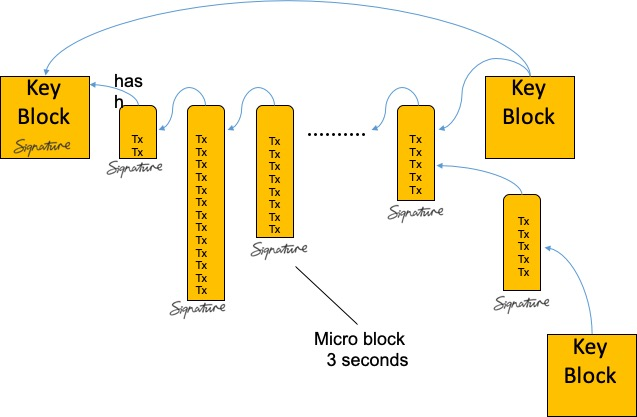
\includegraphics[scale=0.3]{keymicro.jpg}
   \caption{Next generation consensus}
   \label{ng-mining}
\end{figure}

\subsubsection{Fraudulent leaders}

There is only one leader per generation creating micro-blocks. Each key-block
includes the public key of the new leader and consecutive micro-blocks are
only valid if signed with the associated private key. This protects
against third parties trying to post micro-blocks.

A malicious leader, however, could construct forks either by forking directly
from the key-block, or by forking on a micro-block. This could be done to
disrupt the network or to perform double spend attacks. A malicious miner could
also try to produce more micro-blocks than entitled to by fiddling with the
micro-block creation timestamp.

In order to mitigate the risk of a leader forking its own sequence,
there is a mechanism in place to detect and report this by submitting
a Proof-of-Fraud. This is submitted in the next
generation. The leader is punished by not receiving a block reward and
in order to make that possible, block rewards are not immediately paid out but
kept for the duration of 180 blocks.

\subsubsection{Divide and conquer}

Each transaction is a binary of a certain size. Internally both size
and computation are expressed in gas and there is a maximum amount of
gas per micro-block that allows for maximally 300 KB per micro-block.
Thus, an additional advantage of the introduction of micro-blocks is that
instead of a huge block with 180,000 transactions in 3 minutes, we can create
60
reasonably sized micro-blocks of maximally 300 KB  in the same 3
minutes. This has several advantages for network latency and
smaller blocks are easier and faster to gossip through the
network. Moreover, if it takes longer to compute the next key-block we
are not bound to a maximum block size, because we generate new
micro-blocks as long as no key-block has been found.

\section{Transaction types}
\label{sect:transactions}

The aeternity blockchain offers a plurality of different transactions
types, designed to simplify application development for features that are
common or popular in the blockchain sphere. By using smart contracts,
users can develop completely new features themselves, but for already
identified features, a general set of transactions is
provided. These features are spending tokens from one account to
another (Sect.\ \ref{sect:aespend}), naming objects (Sect.\
\ref{sect:aens}), oracles (Sect.\ \ref{sect:aeoracle}), and the
transaction wrappers: generalized
accounts (Sect.\ \ref{sect:ga}), and paying for
(Sect. \ref{sect:payingfor}).
There are also transactions for creating and calling contracts, as
explained in Sect.\ \ref{sect:sophia} and for opening and closing
state channels, deposit and withdraw funds from a state channel as
well as solo closing, slash and force progress to deal with
disputes as mentioned in Sect.\ \ref{sect:channels}.

All transactions are serialized and then cryptographically signed, by default using EdDSA \cite{bernstein2012high}
signatures with elliptic curve Curve25519
\cite{bernstein2006curve25519}. In order to protect against double
spending, each transaction also includes a nonce, which is a stricly
increasing counter connected to the account of the signer.

\subsection{Aeternity accounts}
\label{sect:aespend}

The most basic transaction is a \textbf{spend
transaction} that is used to transfer tokens from one account to
another. An account is identified by the public key of the signer of
a transaction. The spend transaction also serves as the basis for
creating new accounts, by accepting any new recipient public key as a new
account.

Posting a transaction to the chain can fail for many reasons, among
which that the transaction is not correctly signed. But even correctly
signed transactions may fail to become part of the chain.

Each transaction specifies a \textit{fee} that the miner will
     eventually collect when including the transaction in a
     micro-block. This fee can be unattractive, in which case the
     transaction will stay in the transaction pool until it
     expires. Or the fee can be lower than the minimum fee defined by
     consensus, in which case it is an erroneous transaction that
     will be rejected. Including a transaction that is by consensus to be rejected,  such as a
     transaction with lower fee than lowest agreed upon, is called
     fraud. The micro-block is invalid and rejected by
     all other nodes in the network\footnote{Technically posting
       invalid micro-blocks is sometimes possible and a proof-of-fraud
       transaction is posted later to punish the node posting this transaction.}.

Each transaction specifies a \textit{nonce}  to prevent it from replay
attacks \cite{Syverson}. Each new account starts with nonce 1 and as
soon as a transaction with that nonce is accepted on chain, only
transactions with nonce 2 are accepted, etc. A user can post a number
of different transactions with the same nonce in which case it is
non-deterministic which of these transactions will result on chain,
but only one of them will be accepted and the others thereafter
rejected. This can be used as a feature by reposting a
transaction with an unattractive fee with the same nonce and higher
fee. Similarly, a user can post a whole series of transactions with
increasing, but too large nonces. Only when the missing nonce is
posted, all other transactions that possibly remained in transaction
pools are enabled.

\subsection{Aeternity naming system}
\label{sect:aens}

Transferring tokens to a registered name instead of a hard to remember
public key, is a feature that is supported natively by Aeternity.
For example, in a spend
transaction the recipient can be given as a name. For that to work, a
collection of 5 transactions are provided that
resemble internet domain name (DNS) registration.

One of the challenges in name registration is to offer a reasonably
fair system for those that want a specific name. Imagine a user wants
to reserve \textit{emin} as a name. (Since there is currently only one
name space on the aeternity blockchain \textit{chain}, technically the
user wants to claim \textit{emin.chain}.)
A short name of size 4, like \textit{emin}, is a name that
possibly many people like to claim. Just posting this name in a
transaction would reveal to everyone monitoring the
transaction pool that the name is attractive to at least someone. It
is rather easy to
immediately post the same name with a higher fee to have the leader
pick that new transaction instead of the already posted request for
the name \textit{emin}. This is called \textit{front running}, getting
your transaction in front of an already posted transaction by paying a
larger fee. Transaction pools are not under consensus, so there are no
guarantees that front running would work, but if there are many
transaction in the system and one does this within the micro-block
creation time of 3 seconds, there is a fair chance that front running
would work.

In order to defend the users against front running, the first step in
reserving a name is the \textbf{preclaim transaction}. In a pre-claim,
one posts the hash of a combination of the name and a random number
(called \textit{salt}). When the preclaim is accepted, you can
post a claim transaction to obtain the actual name.
The \textbf{claim transaction} is
then used to either immediately obtain the name if the name is long
enough (with current governance values, longer than 12 characters), or to start an
auction. In both cases the
claim transaction reveals the name and the salt.

A fee is paid for the
length of the name, shorter names are more expensive and the auction
is open for a certain period expressed in blocks. For the 4 character
name \textit{emin}, the price starts with 134.6269 AE tokens and the
auction would be open 29760 blocks (approx 62 days) after the last valid bid.

At the moment that someone posts a claim,  the name is known. A potential
front running by quickly posting both a preclaim and a claim for the
same name is mitigated by demanding the preclaim and the claim to be
in different generations. In other words, the original claim can be
added to the generation, whereas the new claim needs to wait until the
next generation.

After that the name is claimed, other users can see this name and
claim it with a higher bid. Each bid must be at least 5\% higher than
the previous bid in order to be a valid bid. Note that the bidder must
have enough tokens and that those tokens are reserved in a claim. The
previous bidder gets the tokens returned as soon as a higher bid is
accepted. This means that this users has the funds available for a
possible next bid.

It is very well possible that two users preclaim the same name with
different salt and then claim, but only one of them is accepted, the
other is not. The rejected name claim transaction is not even seen as
the next bid in an auction, even if the price would be higher. There
is a subtle difference between a bidding claim and the original claim
by the \textit{salt} being zero for a bid and non-zero for an original claim.

After the auction, or for long names instantaneously, the highest
bidder owns the name. An additional
\textbf{update transaction} is needed to point the name to something (for example an
account). Additionally there are a \textbf{transfer transaction} to
change the owner of a name, and a \textbf{revoke transaction} to free the
name.

Names have a specific lifetime and there is an agreed maximum number of blocks one can wait
between a pre-claim and a claim in order to succeed with the claim.
Obviously, registered names expire after a while, unless renewed in time
with the update transaction.

When a name has been assigned to an owner and an update transaction
has pointed this name to an account, then one can use the \textit{name
  hash} of the name instead of an account in, for example, a spend
transaction. The name hash function first converts the name to a unique value using the
internationalized domain name standard IDNA \cite{idna2008}. This makes names
case-insensitive and, in particular, it helps to uniquely map
non-ascii characters. After that, the Blake2b hash is applied. This unique
hash is then part of the transaction and the way the name is
internally represented.
IDNA is used, since there are well known attacks by using names that
look similar to the human eye, but are different.

It is important to realize that the names are part of the blockchain
logic. A user should not trust any third party to perform a name lookup on
chain and then substitute the name by an account. If a user want to
transfer tokens to Emin, the user should put the name hash of \textit{emin.chain} in
the transaction and sign this transaction.


\subsection{Aeternity oracles}
\label{sect:aeoracle}


Smart contracts only operate on data that is on the
blockchain. Oracles are a mechanism to bring external data about
real-world state and events onto the blockchain. Data can either be
obtained from large data sources, real-time data, or heavy computations.

Typical external data may be useful for smart contracts. One can base
a decision in a contract on the state of some external data. This can be sensor data or
news events such as stock data, results of a match, supply chain data,
etc.
Researchers try to address the issue of trust in the authenticity of extrenal data
\cite{zhang2016town,guarnizo2019pdfs, adler2018astraea}, but in
general oracles provide data without robust security guarantees.

Oracles are announced to the chain by a \textbf{register oracle
  transaction}. This specifies in what format the oracle expects its
queries ands in what format it is going to respond. Typically this is
specified as a type signature. The register oracle transaction also
includes the fee of the queries to this oracle. Each query must supply
that fee in order to be answered. The query fee is the economic
incentive for the oracle to provide information.

When an oracle is registered on chain, any user can post a
\textbf{query oracle transaction} with the rightly formatted query.
The oracle supplier monitors the blockchain and will see this
query and post an \textbf{oracle response transaction} with the answer
to the query in the predefined format. In this way,
the data becomes part of the data on the
blockchain. This data can be referred to in a smart contract.

\subsubsection{Data as a service}

External data may come from a large database, possibly also accessible in different
ways, but via the oracle made accessible on the blockchain. Typically
one could think of supply chain data. If supply chain data is
accessible via a trusted oracle, one could post an oracle query for
last transaction on a specific item one ordered. Although the answer
on such a query may be interesting and valuable in itself, the main
purpose of asking for it would be to use it in a contract to transfer
some tokens (goods have arrived in harbour, 20\%  of tokens are
transferred).

The above supply chain data may be anonymous enough to appear on a
blockchain. There is, however a privacy issue, external data that is
put on chain is made public. So, even if there might be an interesting
use case, one must be careful with for example personal data. If one
would have an airline oracle that given a last name and booking
reference returns flight data ``date'', ``from'' and ``destination''
airport, then this becomes public data. Having a contract pay the
travel agent when the oracle returns that the correct date and flight has
been booked, is therefore a bad idea. Even encrypting or decrypting the
data in the contract would be a bad idea, since contract state and
operations are visible.

Moreover, one cannot get paid for the same data twice, because the
first time it is posted, it becomes public. Therefore, typical data
normally is rather anonymous or invaluable to others than involved
parties, or is already/will become public, such as the weather or the
outcome of a match. Point is that one can use data that becomes
available in the future to base contractual decisions upon.

\subsubsection{Off-chain computations}

Oracles can also be used to perform heavy computations off-chain and
then post the actual result on-chain. After all, Sophia and the amount
of gas available would make it impossible to implement a chess
calculator to propose the next good move. Implementing this as an
oracle would work. One queries for a certain position and gets a best
move response. Clearly, the chess hints are already freely available, which harms
this business model more than the fact that hints for specific
positions becomes public data.

\subsubsection{Timing}

Users that post a query would normally want a response rather
quickly. Therefore, they can specify query TTL, either absolute
or relative key-block heights. A relative query TTL of 2 assures
that if the oracle does not answer within 2 key-blocks after the query
is accepted onchain, the query fee is not paid. In fact, an answer that is too
late, will not make it on chain and no contract can use it in a
decision.

Oracles have a specific lifetime, supplied in block height when
registering the oracle. After that block height, queries to the oracle
are no longer resulting in a response. The lifetime of an oracle can
be extended using an \textbf{extend oracle transaction}.


\subsubsection{A lottery example}

An example of the use of oracles and contracts can be illustrated with
a little lottery example. Note that all computation on a blockchain
should be deterministic in order to be able to validate the
results. If not exactly the same, the corresponding state hashes will
differ. As a consequence there is no random number generator in the
Sophia language\footnote{Even if some kind of random function would be
  offered, it would be deterministic and hence have a predictable
  outcome}.

Running a simple lottery in which users buy a ticket and after a while
one draws one of the tickets as the winner, is somehow depending on
some kind of fair randomness. If the number is known or computable at
the start of the buying process, one might be able to figure out what
ticket to buy to win the lottery. But if we close the lottery and then
ask an oracle for a random number, then a trusted, but disconnected
computation can be used to draw the winner.

So assume there is such an oracle, monitoring the chain and registered
with a reasonable query fee covering for its cost of operation. The
oracle has an identifier, for the example say
\textit{"ok\_shEHMV8Q2F1HR86pcyF7DYpudg8hnvJwJuVE3berWpbktnL2R"}.
We can now write a Sophia contract that takes this oracle identifier
as input of its initialization and uses it for random numbers in the
lottery game.

\begin{verbatim}
include "List.aes"

contract Lottery =

  record state = { participants : list(address),
                   price_sum : int(),
                   close_height : int(),
                   oracle : oracle(int, int),
                   query : option(oracle_query(int, int))  }

  entrypoint init(rand : oracle(int, int)) : state =
    { participants = [],
      price_sum = 0,
      close_height = 0,
      oracle = rand,
      query = None }
\end{verbatim}

The contract stores a list of participants in its state, a price sum
that increases for each ticket bought, a closing height after which no
new tickets can be purchased. The initial closing height is zero,
because initially there is no ongoing lottery. The state also contains
an oracle and an optional query. This query will be instantiated when
the lottery is closed and a ticket is drawn.

The creator of this contract may now start the lottery by supplying a relative closing height,
for example, 20 key-blocks from that the transaction gets on chain;
approximately one hour. Any user can then buy a ticket.
\begin{verbatim}
  stateful payable entrypoint start(n : int) =
    require( Call.caller == Contract.creator, "not creator" )
    require( state.price_sum == 0, "lottery ongoing" )
    require( n > 1, "block in future")
    put(state{ participants = [],
               close_height = Chain.block_height + n })

  stateful payable entrypoint buy() =
    require( state.close_height > Chain.block_height, "lottery closed" )
    require( Call.value == 10, "price ticket 10" )
    put(state{ participants = Call.caller :: state.participants,
               price_sum = state.price_sum + 8 })  // we take 20%
\end{verbatim}
Note that a lot of conditions are checked, resulting in abortion of
the contract when falsified. In general, making the contract safe
requires thinking through a large number of possible scenarios in
which things may not work out as expected.
For example, if no users buy a ticket\footnote{The price of the ticket
is set to $10$ aettos instead of a more realistic  $10\_000\_000\_000\_000\_000$ to
make the code more readable}, the contract creator must be
able to restart the lottery at a later time, but the creator should
not be able to restart as soon as there are participants. Similarly,
one should not allow participants to buy tickets when the lottery is
closed.

The keyword \verb+payable+ expresses that we expect the participants
to add a token amount to the contract call transaction, which is
checked by comparing \verb+Call.value+. Similarly, the contract
creator needs to pay something into the contract to cover the oracle query
fee\footnote{Note that there is no check in the contract that it has
  enough funds to query the oracle after starting a lottery. The
  participants are at risk here} in case there are too few
participants.

When the closing height is reached, someone, most likely the creator
of the contract, asks the oracle to draw a number between 1 and the
number of participants. This call returns the query., such that anyone
can monitor the chain to see if the query has arrived. When that's the
case, the winner, or anyone else, can call the claim function, which
will transfer the price sum to the winner.
\begin{verbatim}
 stateful entrypoint draw() : oracle_query(int, int) =
     require( Chain.block_height > state.close_height, ongoing lottery" )
     require( state.price_sum > 0, "no ongoing lottery" )
     require( state.query == None, "already drawn" )
     let q =
        Oracle.query(state.oracle, List.length(state.participants) - 1,
                     Oracle.query_fee(state.oracle),
                     RelativeTTL(5), RelativeTTL(480))
     put(state{query = Some(q)})
     q

  stateful entrypoint claim() : option(address) =
    switch(state.query)
        None => abort( "no drawing" )
        Some(query) =>
          switch( Oracle.get_answer(state.oracle, query))
             None => abort("waiting for query")
             Some(winner) =>
               let winner_account = List.get(winner, state.participants)
               // Spend to winner
               Chain.spend(winner_account, state.price_sum)
               put(state{ price_sum = 0, query = None })
               Some(winner_account)
\end{verbatim}

The reason to make it possible for anyone to call these functions is
to ensure that the contract creator can force progress to start a new
lottery and the winner to be able to claim even if the contract owner
is not around. The TTLs in the query assure that the oracle has
approximately 15 minutes to answer, long enough to even get it out
in busy times. Within a day one then has to claim the price sum,
otherwise, because the query answer is then no longer on chain.

This contract is far from fully secure, but illustrates an example of
how oracles and contracts can be used together. An easier way to
get a reasonable random number is to use the hash of the key-block at
closing height.




\subsection{Generalized accounts}
\label{sect:ga}

Generalized accounts are a way to provide more flexibility to signing
transactions. Both the nonce handling and the signature checking are
done by a smart contract that is attached to the account. This can,
for example, be useful when one would allow users to sign transactions with
other cryptographic primitives than the default\footnote{Some hardware
  devices may be restricted to other cryptographic signing algorithms
  than the default on the aeternity blockchain.} EdDSA as mentioned in
Sect.\ \ref{sect:transactions}.

If a user wants to have a generalized account, then this user must
provide a smart contract in a \textbf{attach transaction}. This
contract is thereafter attached to the given account. The contract
must have an authentication function that returns a boolean whether or
not authentication is successful. The attach transaction itself is
just like all previously mentioned transactions signed in the default
way. It turns a normal account into a generalized account, and
\textit{there is no way back}.

When an account is a generalized account, any transaction can
be wrapped in a so called \textbf{meta transaction}. That is, one
prepares an ordinary transaction in the usual way, but with a nonce set to
zero. After that, one adds additional fee, gas and authentication data to
run the smart contract. When this transaction is processed, the
authentication function in the smart contract associated with the
account is called with the provided authentication data as input. If
the authentication fails the transaction is discarded, otherwise its
inner transaction is processed.

The following smart contract is an example that allows signing with
the ECDSA algorithm \cite{johnson2001elliptic} and the popular elliptic curve
Secp256k1, used for example by Bitcoin and Ethereum
\cite{bos2014elliptic, mayer2016ecdsa}.

\begin{verbatim}
contract ECDSAAuth =
  record state = { nonce : int, owner : bytes(20) }

  entrypoint init(owner' : bytes(20)) = { nonce = 1, owner = owner' }

  stateful entrypoint authorize(n : int, s : bytes(65)) : bool =
    require(n >= state.nonce, "Nonce too low")
    require(n =< state.nonce, "Nonce too high")
    put(state{ nonce = n + 1 })
    switch(Auth.tx_hash)
      None          => abort("Not in Auth context")
      Some(tx_hash) =>
        Crypto.ecverify_secp256k1(to_sign(tx_hash, n), state.owner, s)

  function to_sign(h : hash, n : int) : hash =
    Crypto.blake2b((h, n))

\end{verbatim}

The contract is initialized by providing the public key used for
signing and the nonce (in the contract state) is set to 1. The
authentication function takes two parameters, the nonce and the signature.
The authorization function checks that the nonce is correct, and then
proceeds to fetch the TX hash from the contract environment using
\verb+Auth.tx_hash+. In this example the signature is for the Blake2b
hash of the tuple of the transaction hash and the nonce). The
authorization finally checks that the private key used for signing the
hash was from the owner.


By attaching this contract to an aeternity account, users can sign
aeternity transactions with their bitcoin private key. They need to
keep track, of course, what nonces they have used for this contract,
to provide the right next nonce.

\subsubsection{Security considerations}

Before the authentication is performed, there is no account that one
can charge for the computational effort of running the authentication
function. After all, anyone could wrap a transaction in a \textbf{meta
  transaction} and submit it. It would be an easy attack to empty a
generalized account if the account had to pay for failed authorization
attempts. So, the gas for authentication is only charged when
successful. This opens up for another unpleasant attack.

Since there is no cost involved for the user to run an authentication
function, but the miner needs to spend execution cycles, one could
potentially write a complex function as authentication function and
extract resources from a miner by calling one's own authentication
function with failing input data. This is mitigated by not allowing
expensive chain operations in an authentication call. Moreover, miners
are free to implement any sophisticated rules for accepting
transactions in their mining pool, such that they can reject this
behaviour when observed.

Using different signature algorithms is only one of many possible uses
of generalized accounts. Other uses cases can be multi-sig, spending
limits (per week/month), limiting the transaction types, and more. For
these applications smart contracts have to be written. Utmost care
needs to be taken when implementing the authorization
function in these smart contracts. If the contract does not enforce
integrity checking or replay protection, then it will be vulnerable to
abuse.


\subsection{Financing transaction costs}
\label{sect:payingfor}

In order to make users enthusiastic about a blockchain application,
one may want them to try it for free. However, there are always costs
involved for transaction and gas. This means that a new user has to
buy tokens at some exchange to pay for the fees. This can be considered
a hurdle for adoption. Of course, one can ask a user for an account and put
some tokens on it, but then those tokens can be used for anything.
The aeternity solution is more powerful and can be used to pay for
just specific transactions. It can be used to pay for both transaction
fee and gas cost of a contract call.

Assume a game played via a contract on the blockchain. One interacts
with the game, by calling the contract. In order to get more users for
the game, the game provider could make an App that visualizes
the game and asks for a next move. This App could automatically create
an aeternity account, even without the user being aware of it. This
account can be used to sign transactions on the blockchain, but there
are no tokens in the account. This move is then encoded in a
transaction signed by the players account in the App. The transaction
is submitted to the game provider, who inspects it to see that this
is indeed a move in the game and wraps it in a \textbf{payingfor
  transaction} signed by the game provider. The gas and fee are now
paid by the game provider's account.
Clearly this is also a way to have some trustful cross-chain
activity. The App user could provide the game provider with funds on a
different blockchain.

One can pay for any transaction apart from the payingfor transaction
itself. So even a generalized accounts meta transaction can be paid
for, as long as it recursively does not contain any other payingfor
transaction.

\section{Scaling with state channels}
\label{sect:channels}

The NG technology mentioned in the previous section improves
scalability by faster preliminary confirmation times for
transactions. It also lifts the restriction of a maxiumum number of transactions in a
generation; when it takes longer to produce the next key-block,
additional micro-blocks can be generated containing new transactions.
This benefits throughput and confirmation times. But if parties really
want confirmation times in milliseconds and perform more advanced
computations than the total amount of gas in a micro-block would
allow, then state channels come to the rescue.

Conceptually one can regard a state channel as an agreement between
two parties to build a chain of state changes on the side. Only the
agreeing parties have access to this chain in the so called
\textit{state channel}. The parties agree the initial
state of this chain. Typically, the state would
contain some initial accounts for the involved parties in which they
reserve some tokens from the aeternity blockchain for transactions in
the channel. Then they post a joinedly signed transaction on-chain to
confirm that this is the initial state.
The amounts the initial amounts are then reserved on-chain and cannot
be used on-chain until they are released.

Apart from initial amounts,
they also post the hash of the channel state tree: the state the
parties do agree upon. By only submitting the hash, the actual state
is kept private to the channel, both parties know, but they need not
reveal it.

If only accounts are used in a state channel, one can consider it a
payment channel. However, one can also agree upon a contract in the
channel, either initially, or added later. In this way, one can also
perform contract calls to update the state of the channel.

The state representation is determined by the state channel
implementation and different implementations may in theory use each
their own representation. The state hash is what is visible on-chain
and what parties agree upon in their transactions.
In case of dispute resolution, the
latest agreed, mutually signed, state hash can be posted to the aeternity blockchain.

\subsection{On-chain and off-chain transactions}

In a state channel impementatioin users communicate peer-to-peer with
each other, using mutually signed transactions that include state
hashes. In this way parties agree upon a state, without any
mining involved. Instead of creating key or micro-blocks, the transactions are just
directly applied to update the state. Only states
jointly agreed upon are recorded. This also
means that there are no transaction or gas costs involved\footnote{In a state
channel parties can agree to have a kind of transaction cost, but it
is not the default implementation} and most notably that a transaction
is confirmed as quickly as both parties can sign it. This confirmation
time can therewith be reduced to milliseconds.

A typical use-case for a state channel, or rather a payment channel, is a subscription model, for
example a coffee ``account'' with 25 cups of coffee. Each time one
orders a coffee, the coffee shop
creates a transaction to update the state and both shop
and customer sign this transaction. They agree upon the new state.
Since it would be annoying to have to wait 3 minutes or even 3 seconds
on the payment of a cup of coffee, it is a good example for off-chain
processing. At the same time, it also addresses privacy concerns,
since only the involved parties and not all the users of the
blockchain need to monitor the customers coffee consumption.

Scaling is achieved by performing transactions \textit{off-chain},
i.e.\ transaction in the channel. One starts with an \textit{on-chain}
transaction agreeing and verifying a starting state and balance. After
that many transaction can be performed without involving the aeternity
blockchain. A coffee shop could have thousands of customers, all buying coffee and none of
this puts transaction pressure on the blockchain. Only after
terminating or topping up of a subscription, a new on-chain
transaction should be recorded. Having a thousand cups of coffee paid
per second is no technical limitation, but possibly hard to achieve as
a business.

The coffee subscription only includes two accounts and off-chain
payments from one of these accounts to the other.
Notably one
can create contracts in a channel or refer in a channel to contracts
created on the blockchain. We discuss contracts in Sect.\
\ref{sect:sophia}, but one use case is to implement a game playing
contract (e.g.\ tic-tac-toe) and refer to that contract when playing the
game in a channel. In such use-cases it is also an advantage to be
able to play quickly and not having to wait 3 seconds before once move
is included in a transaction.

\subsection{Disputes}

A state channel requires both parties to sign each state to make
sure the state is agreed upon. Typically a state channel can be closed
under mutual agreement and then a closing transaction is used to
re-distribute and return the reserved balances to the on-chain
accounts. Another way to extract reserved funds from a state channel
is to mutually agree upon a withdraw from the channel to an account of
one of the parties. Typically, topping up a subscription would be done
in combination with the coffee shop withdrawing part of the funds in
the channel.

But there might be disputes. For example, a customer
could decide not to cancel a subscription, but keep an empty account
in the state channel for ever. This is disadvantageous for the shop,
because it cannot extract the funds from the already paid coffee in
mutual agreement. For this reason, there is a solo close transaction,
a way for one party to close the channel on-state and use the last
signed and agreed state as a proof on how the funds should be divided.

Clearly, there is plethora of scenarios in which one can try to
cheat. One could buy a coffee off-chain and at the same time solo
close the channel on-chain. That would mean a free coffee. Therefore,
funds are not immediately returned after a solo close, but kept for a
certain period, called a \textit{lock period}. During this period the
other party can post a transaction to refute this claim and show a
later state obtained by a mutually signed transaction (the one after
buying the additional coffee). Which then again could possibly be
refuted, etc.

Dealing with disputes is a considerable part of the logic and
implementation of state channels. This becomes even more evident in
the context of using contracts in a channel. A contract may be build
in such a way that it re-distributes balances after a certain state has
been reached. Imagine the above mentioned tic-tac-toe game contract,
where the funds are re-distributed only after that one party has
won. It could then be beneficial for a party to quit the
game when loosing and solo close, or to simply refuse to sign the last
transaction.

Quitting when one expects to lose
harms the other party, because there is no next state that is more
beneficial than the initial state. For this purpose the other party
can then force progress the contract and move to the winning
state. That is, the party can perform a contract call and show that it
ends up in state that can be claimed the actual final state for which
the channel should be closed. This force progress requires more than
just the state hash, here a state has to be revealed that can be used
by the aeternity blockchain to execute the next step in the
contract. This requires to folllow a predefined format for the state trees.

Clearly, a number of different counter
measures are present for the other party in case a malicious force
progress transaction is posted. It is also clear that the state of the
state channel has to be made public (at least partly) to settle a
contract dispute in a force progress transaction.

Users should keep in mind that, by using a state channel, they trade
transaction efficiency and lower transaction fees for some reduction in
safety.
The on-chain transactions are under consensus, but on top of that,
several implementations can be build that offer access to the state
channel with their own implementation logic. For users of a state
channel, it is important to know and understand the limitations of
these off-chain implementations. For example, whether they monitor
on-chain transactions that influence the state channel, such as a
direct solo-close transaction on chain.
Despite, a plurality of dispute handling primitives that are offered to
mitigate the problems dealing with potentially malicious parties,
users may not have the knowledge to use these primitives without a
third party implementation. Therefore it is important to users to understand
whether and how they are implemented.

\section{Sophia smart contracts}
\label{sect:sophia}

Smart contracts \cite{szabo1996smart,hhz007} are
programs on the blockchain that can perform tasks with the data on that
blockchain. Typically contracts have state (data), which is recorded on the
chain. A call to a function in the contract results in a return value
and updated state, both put back on the chain as a result of the
call.

Smart contracts are written in a programming language and for the
aeternity a totally new language has been designed, called
\textit{Sophia}. There is a compiler that compiles Sophia contracts to
byte code that is executed by the virtual machine part of the
blockchain.

Contracts are put on chain by contract create
transaction, specifying their byte code and data to compute the
initial state. A contract on chain is called by contract call transactions\footnote{in
  Aeternity  contracts are executed by a call, there is no
  mechanism to automatically progress computation.}. Each contract
creation and contract call requires computation effort and the user is paying
for that effort by paying for \textit{gas}. Each operation is
associated with a certain amount of gas and the total used gas is paid
for. The user specifies how much gas is provided in the transaction. A
surplus is returned. If there is too little gas provided, the
transaction is accepted (it is recorded
on the chain), and the user pays for transaction fee and gas,
but the contract computation has failed and its state is unchanged.

Smart contracts are an active research field
\cite{DBLP:journals/corr/abs-1710-06372} and a substantial amount of
  effort goes in to studying the verification and validation of smart contracts
  \cite{magazzeni2017validation,bhargavan2016formal}.

There are two major technical challenges for smart contract
implementations. The first challenge is to make the contracts
execute fast without requiring too many resources. In a blockchain
implementation, contract execution is performed in a
\textit{virtual machine}. This is an execution engine with formally
defined semantics, such that all implementations perform exactly the
same computation steps, with exactly the same result and charging
exactly the same amount of gas. The aeternity blockchain defines two virtual
machines, the AEVM, compatible to the Ethereum blockchain, and the more
efficient FATE virtual machine.

The second challenge is to design a language to express contracts in
such a way that one can understand and reason about the contract
both as a human, but also mechanically by computer programs. The
language should by design protect contract designers against
vulnerabilities that can be exploited. Sophia is a functional language
to accommodate for these properties. It is designed as a contract
language with security and user comfort in mind. In particular,
vulnerabilities in contracts in other languages
\cite{atzei2017survey,mehar2019understanding,delmolino2016step} have been studied with the goal to
avoid the possibility to make such mistakes in Sophia.

\subsection{The Sophia language}

\todo{Mention calling a contract  from a contract}

Sophia is a functional language \cite{hughes1989functional}.
The main unit of code in Sophia is the \textit{contract}.
A contract implementation, or simply a contract, is the code for a
smart contract and consists of a list of types, entrypoints and local
functions. Only the entrypoints can be called from outside the
contract.   A \textit{contract instance} is an entity living on the
block chain (or in a state channel). Each instance has an address that
can be used to call its entrypoints, either from another contract or
in a call transaction.  A contract may define a type \texttt{state}
encapsulating its local state. When creating a new contract the
\texttt{init} entrypoint is executed and the state is initialized to its
return value.


\subsubsection{Dutch auction contract}

As an example, let us consider an auction contract.  In such an
auction contract, a user could auction an object in the real world by
creating and posting a contract to the blockchain, using a \textbf{contract
create transaction}. Let us assume that
this is a Dutch auction, then the initial price
would be set high and for each new key-block that is mined (representing
time) the price is decreased. Someone buys the object by calling a
\texttt{bid} function. When this bidding \textbf{contract call transaction} executes,
the contract computes the price on that height; if the caller has
supplied enough funds in that call, the seller is paid, the
bidder is charged (possibly refunded the extras) and the contract
enters a non sellable state for the object. The next bidder will fail
the call and only pays for transaction costs, not for the object.

The complete Sophia code for a Dutch auction is presented here:

\begin{verbatim}
contract DutchAuction =

  record state = { amount : int,
                   height : int,
                   dec    : int,
                   sold   : bool }

  entrypoint init(price, decrease) : state =
    { amount = price,
      height = Chain.block_height,
      dec    = decrease,
      sold   = false }

  stateful payable entrypoint bid() =
    require( !state.sold, "sold"  )
    let price = demanded_price()
    require( Contract.balance >= price, "not enough tokens" )
    Chain.spend(Contract.creator, price)
    Chain.spend(Call.origin, Contract.balance)
    put(state{sold = true})

  function demanded_price() : int =
    state.amount - (Chain.block_height - state.height) * state.dec

\end{verbatim}

The contract languages and hence the evaluation in the virtual
machine, must have access to blockchain primitives like the height of
the chain and caller accounts. Typically, all blockchain
primitives are available from within a contract.

Note that the contract create transaction includes the contract
byte code, not the source code, together with information on
which version of the compiler is used. Compiled for FATE this contract
results in 254 bytes, whereas compiled for the AEVM 2092 bytes are
needed. The gas needed to compute the initial state is 240 for FATE compared
to 741 for the AEVM.

The \texttt{init} function is called when the contract is created to
compute the initial state of the contract. The \texttt{init} function
is not part of the byte code, such that it cannot accidentally be
called again. If one wants to reset the state, this has to be
explicitly programmed to avoid expensive exploits
\cite{suiche2017280}.
The contract designer also has to explicitly mention whether the
state of the contract is changed in a call (using the
\texttt{stateful} keyword).
Entrypoints can be called from outside the contract, whereas functions
are only accessible from within the contract.

The keyword \texttt{payable} is added to explicitly state which
function calls expect to come with additional tokens in the contract
call transaction. These tokens are added to the contract balance
before the call is made. If, however, the call is reverted by a failing
\texttt{require}d condition, then the provided tokens are returned.

The transparency of the blockchain guarantees that it is verifiable
that the first valid bid on chain\footnote{The blockchain
  does not guarantee that the first one posting a valid bid becomes
  the first one on chain.} is correctly paying the right
price. Moreover, it is verifiable that the bidding call transactions accepted later are
only charged a transaction fee and the cost of execution.
The sale conditions are transparent, but whether the actual object ever
arrives is outside the scope of the blockchain

\subsection{The FATE virtual machine}
\label{sect:fate}

The Fast aeternity Transaction Engine (FATE) VM uses transactions as
its basic operations and operates directly on the state tree of the
æternity chain. This enables native integration with first class
objects such as oracles, the naming system, and state channels since
those are all managed by specific types of transactions described on
the protocol level. FATE is a simple-to-use machine language, superior
to the more traditional byte-code virtual machines currently used on
other platforms. It enables easier, safe coding, faster transactions,
and smaller code sizes. It is custom-built to seamlessly integrate
with the functional smart contract language Sophia.

\subsubsection{More secure}

Every operation and every value is typed. Any type violation results in
an exception and reverts all state changes. This prevents people to
circumvent the compiler and write or modify their own FATE code to use
type violations as an attack vector.

The instruction memory is divided into functions and basic
blocks. Only basic blocks can be indexed and used as jump
destinations. This is a precaution to be unable to jump to arbitrary
positions in memory. It also carefully fit FATE's function style by
having function calls instead of jumps. Moreover, data and control
flow are separated, one cannot possibly modify the running
contract, since the code memory cannot be written to.

FATE is “functional” in the sense that “updates” of data structures,
such as tuples, lists or maps do not change the old values of the
structure, instead a new version is created.  FATE does have the
ability to write the value of an operation back to the same register
or stack position as one of the arguments, in effect updating the
memory.

FATE solves a fundamental problem programmers run into when coding for
Ethereum: integer overflow, weak type checking and poor data
flow. FATE checks all arithmetic operations to keep the right meaning
of it. Integers cannot overflow, since FATE uses unbounded integer
arithmetic (cf.\ Bignums \cite{serpette1989bignum}). Floats are not
part of the language, avoiding a bunch of issues associated with
floating point arithmetic. Also you cannot cast types (e.g\ integers to booleans). This makes
FATE ultimately a safer coding platform for smart contracts.

\subsubsection{More efficient}

FATE uses high level instructions. There are instructions to operate
on the chain state tree in a safe and formalized way. Likewise the
virtual machine has high level support for most of the transactions
available on the aeternity blockchain. There are operations such as
`ORACLE\_CHECK\_QUERY' for querying an oracle or `AENS\_CLAIM' for
claiming a name.

Having higher level instructions makes the code
deployed smaller and it reduces the blockchain size. FATE contracts
use on average ten times less space than the same contract compiled to
the AEVM, the Ethereum compatible VM. At the same time, it performs on
average much faster and uses therefore less gas.

FATE byte code looks in itself as a readable program. For example,
the bid function of the Dutch auction contract compiles to
this code:

\begin{verbatim}
FUNCTION bid( ) : {tuple,[]}
  ;; BB : 0
          ELEMENT a 3 store1
          NOT a a
          JUMPIF a 2
  ;; BB : 1
          ABORT "sold"
  ;; BB : 2
          CALL "(h:p"
  ;; BB : 3
          POP var1
          BALANCE a
          EGT a a var1
          JUMPIF a 5
  ;; BB : 4
          ABORT "not enough tokens"
  ;; BB : 5
          CREATOR a
          SPEND a var1
          BALANCE a
          ORIGIN a
          SPEND a a
          SETELEMENT store1 3 store1 true
          RETURNR ()
\end{verbatim}

The notion \verb+BB+ stands for basic block and jumps are always to
such a basic block. Note that for example `CREATOR', `SPEND' and
`BALANCE' are native instructions used in basic block 5. The
instruction \verb+ CALL "(h:p"+ in basic block 2 looks a bit cryptic for a call to  the
function \verb+demanded_price()+. Each function name is hashed to 4
bytes that are printed as a string.

Both memory constraints and computation efficiency are important to
enable smaller contracts to also be run on IoT devices
(cf. \cite{ellul2018alkylvm}) as well as to be able to get more
computation into a micro-block.

\section{Future ambitions}

The \blockchain\ went live on November 28th, 2018. For the curious reader,
there is a timestamp in each block and the first mined key-block has timestamp
``1543373685748'', which is the time in milliseconds using POSIX time. Since
that first date, 3 major protocol updates have successfully be applied,
enriching the \blockchain\ with new features. The new protocols are effective
at a certain height and the software supports the old protocol under that
height and the new protocol from that height. Each protocol is referred to by
name for ease in communication with developers of blockchain applications:
\textit{Roma}, effective at height 0, \textit{Minerva}, effective at height
47800, \textit{Fortuna}, effective at height 90800, and \textit{Lima},
effective at height 161150.

In the future, there will be more protocol upgrades with additional features,
some of which we are going to outline in this section.

\subsection{Formal verification}

Over the course of its existence Ethereum has had many big flaws on deployed
contracts uncovered and abused. Some of these were simple developer errors and
others very subtle due to the complexity of both the EVM and Solidity.

Formal verification is one of the approaches to prevent these problems by
allowing code to be proven correctly with regards to a given specification.
Formal verification is used in many areas where high assurance is of vital
importance, e.g. cryptographic systems.
Take the parity multi-sig contract flaw, which allowed anyone to destroy one of
the libraries used by the multi-sig contract rendering it useless, as an
example. A formal specification of this contract could include the assumption
that destruction functions can only be called by authorized accounts or not at
all. Checking this specification against the code would then have raised an
error. But there is certainly still the problem of writing good specifications.

Since Sophia was written with formal verification in mind, we have laid most of
the ground work required to provide these tools. Together with Sophia being a
functional language, this should prevent many classes of bugs plaguing Solidity
smart contracts.

\subsection{Native tokens}

The ERC-20 standard, which specified an interface for fungible tokens, was
arguably one of the biggest drivers of adoption for Ethereum. With that came
the ability for anyone to design and test economic systems, which was a great
catalyst for the innovation happening on Ethereum. A big drawback of the token
contracts deployed was and still is the requirement to pay gas and thus own
Eth, which can be a major hurdle for users, who don't necessarily want to own
any Eth or even know what that is. In addition to that, interacting or
integrating with token can be a pain, especially since the interface evolved
over time and if upgradability was not baked into the contract there are only
very clumsy upgrade paths for old contracts.

To address these drawbacks, \aet\ will make tokens native to the blockchain.
That opens the way to be able to use tokens to pay transaction fees, which
frees users from the requirement to own any other tokens. It will make usage
cheaper since the basic token logic and storage can be optimized in the virtual
machine. Finally, this will allow tokens to benefit from updates and upgrades
for free, without needing complex upgrade strategies.

\subsection{Computational integrity}

Computational integrity assures that a given function was computed correctly.
This could mean that a coin transfer correctly deducts coins from one account
while adding it to another or the correct execution of a smart contract call.
Currently assuring these correct executions is done by miners and node
operators via complex consensus rules. It also requires everyone who wants to
check the correct execution to re-run the full computation, which could be very
costly.

There are different ways that allow checking the integrity of a function
execution but we are going to assume that the prover, the agent running the
computation and trying to prove that they executed it correctly, can generate a
succinct proof. Succinctness implies that checking the proof is
computationally less expensive than actually re-running the computation. This
proof can then be read and validated by another party, the verifier, who wants
to check the integrity of the computation.

The existence of such primitives then allows scaling, since checking the
proof takes less resources than running the computation. Additionally, these
proofs can be generated in such a way that the function itself can be private,
while still being verifiable by a third party, which would be a big gain in
privacy.

Sophia already comes with some primitives to write efficient proof verifiers
and in the future we want to integrate these primitives even further into the
\aet\ protocol, to make it faster and private.

\subsection{Scaling}

The Bitcoin-NG consensus described in section \ref{sect:mining} allows us to
handle around 120 transaction per second which is sufficient to process
everything almost without delay or block congestion at the time of writing.
But in a future where millions of people want to use \aet\ we will need higher
throughput. One partial solution, state channels, are already available today
and will become more relevant as usability improves.

Besides state channels exist many other different approaches, which can be used
alongside. The most obvious solution is to improve the consensus algorithm in
such a way that it can handle higher throughput and there are already many
other consensus algorithms, which can improve on Bitcoin-NG.

Another direction to go is to split the blockchain into distinct parts, which
is also common for databases. These parts are then called shards and each one
will then be responsible for only a subset of all available transactions.
Dividing up the work like this would then offer each shard more room to scale
just by virtue of only having to handle a fraction of the previous load. Shards
will still have to communicate with each other, which is a possible bottleneck,
and have to know of each others existence. But overall the system could present
a big gain in throughput.

The third widely researched solution are then side-chains, app-chains or
child-chains.
Unlike sharding, side-chains do not divide a global state space but each
one has its own state. The idea of this approach is to have many specific,
maybe even single purpose, chains which do not necessarily have to know of each
other. The name side-chain usually implies that they are
pegged to some sort of main or parent chain, which can be thought of as a
communication hub. Side-chain then imply that each app could get its own chain,
thus only having to handle transactions for this one app and not be concerned
with all the other applications. This in turn would then allow each app much
more throughput and maybe even specific optimizations.

All the solutions described here offer different trade-offs but could certainly
be used in tandem. \aet\ will most likely take elements from all the presented
approaches in order to meet demands by users.


%\input{conclusions.tex}

\bibliographystyle{acm} \bibliography{paper}

\end{document}
